% template by Natalia Chernov for the University of Oldenburg

\documentclass[xcolor=table,9pt,aspectratio=169]{beamer}

\usepackage[utf8]{inputenc}

\usepackage{amsmath}
\usepackage{anyfontsize}
\usepackage[english,ngerman]{babel}
\usepackage[autostyle]{csquotes}
\usepackage{datetime}
\usepackage{enumitem}
   \def\labelitemi{--}
   \def\labelitemii{--}
   \def\labelitemiii{--}
\usepackage{helvet}
   \renewcommand{\familydefault}{\sfdefault}
\usepackage{hyperref}
   \urlstyle{same}
\usepackage{lipsum}
\usepackage{listings}
\usepackage{lmodern}
\usepackage{multicol}
\usepackage{multirow}
\usepackage{smartdiagram}
\usepackage{tikz}
\usepackage{xcolor}

\definecolor{uolblue}{RGB}{0,62,107}

\definecolor{blue1}{RGB}{0,78,159}
\definecolor{blue2}{RGB}{0,171,217}
\definecolor{blue3}{RGB}{91,197,242}
\definecolor{blue4}{RGB}{161,217,248}

\definecolor{green1}{RGB}{0,120,120}
\definecolor{green2}{RGB}{0,168,121}
\definecolor{green3}{RGB}{148,193,28}
\definecolor{green4}{RGB}{199,211,0}

\definecolor{orange1}{RGB}{213,59,10}
\definecolor{orange2}{RGB}{238,113,0}
\definecolor{orange3}{RGB}{243,145,0}
\definecolor{orange4}{RGB}{253,195,0}

\definecolor{gr}{RGB}{191,191,191}
\definecolor{grcode}{RGB}{190,190,190}

\lstdefinestyle{mystyle}{
   backgroundcolor=\color{grcode},
   commentstyle=\color{blue1},
   numberstyle=\tiny\color{blue1},
   basicstyle=\ttfamily\footnotesize,
   breakatwhitespace=false,
   breaklines=true,
   captionpos=b,
   keepspaces=true,
   numbers=left,
   numbersep=5pt,
   showspaces=false,
   showstringspaces=false,
   showtabs=false,
   tabsize=2
}

\setbeameroption{hide notes}
% \setbeameroption{show only notes}
% \setbeameroption{show notes on second screen=right}

\setbeamertemplate{frametitle}{\color{uolblue}\fontsize{12}{20}\selectfont{\insertframetitle}}

\pgfdeclareimage[width=0.145\paperwidth]{logo}{figures/logo_uol_negative}
\pgfdeclareimage[width=0.072\paperwidth]{logo_small}{figures/logo_uol_negative}

\defbeamertemplate*{background canvas}{default_page}{
\begin{tikzpicture}
   \useasboundingbox (0,0) rectangle (\the\paperwidth,\the\paperheight);
   \filldraw[fill=uolblue,fill opacity=1,draw=none] (0,0) rectangle (0.119\paperwidth,\the\paperheight);
   \filldraw[fill=blue2,fill opacity=1,draw=none] (0.119\paperwidth,0) -- (0.119\paperwidth,0.565\paperheight) arc (117.2:180:0.6\paperwidth) -- cycle;
   \pgftext[at=\pgfpoint{10}{\the\paperheight-11.5},left,top]{\pgfsetfillopacity{1}\pgfuseimage{logo_small}};
\end{tikzpicture}
}
\defbeamertemplate*{background canvas}{titlepage_image}{
\begin{tikzpicture}
   \useasboundingbox (0,0) rectangle (\the\paperwidth,\the\paperheight);
   \filldraw[fill=uolblue,fill opacity=1,draw=none] (0,0) rectangle (\the\paperwidth,\the\paperheight);
   \filldraw[fill=blue2,fill opacity=1,draw=none] (\the\paperwidth,0) -- (\the\paperwidth,0.66\paperheight) arc (90:180:0.6\paperwidth) -- cycle;
   \pgftext[at=\pgfpoint{14}{\the\paperheight-17.5},left,top]{\pgfsetfillopacity{1}\pgfuseimage{logo}};
\end{tikzpicture}
}
\BeforeBeginEnvironment{frame}{
   \setbeamertemplate{background canvas}[default_page]%
}
\makeatletter
\define@key{beamerframe}{titlepage_image}[true]{
   \setbeamercovered{invisible}%
   \setbeamertemplate{background canvas}[titlepage_image]%
}
\makeatother%

\setbeamertemplate{footline}{
   \leavevmode
   \hbox{
   \hspace*{.025\paperwidth}\begin{beamercolorbox}[wd=.094\paperwidth,ht=2.25ex,dp=1ex,left]{}
   ~

   \vspace*{.042\paperheight}
      \fontsize{4.4}{5.9}\selectfont\color{white}\textbf{Slide \insertframenumber}\newline\insertdate
   \vspace*{.026\paperheight}
   \end{beamercolorbox}
   \hspace*{.05\paperwidth}\begin{beamercolorbox}
   [wd=.79\paperwidth,ht=2.25ex,dp=1ex,left]{}
   ~

   \vspace*{.042\paperheight}
      \fontsize{4.4}{5.9}\selectfont\color{black}\textbf{Distributive Justice and Reference Points}\newline\color{gray}\insertauthor~--~Faculty IV, Department of Philosophy
   \vspace*{.026\paperheight}
   \end{beamercolorbox}
   }
   \vskip0pt
}

\setbeamerfont{title}{size={\fontsize{22}{25}}}
\setbeamerfont{subtitle}{size={\fontsize{12}{14}}}
\setbeamerfont{author}{size={\fontsize{9}{11}}}
\setbeamerfont{date}{size={\fontsize{9}{11}}}
\setbeamercolor{title}{fg=white}
\setbeamercolor{subtitle}{fg=white}
\setbeamercolor{author}{fg=white}
\setbeamercolor{date}{fg=white}
\setbeamercolor{color_Logo-Platzhalter}{fg=white,bg=gray!40}

\defbeamertemplate*{title page}{customized}[1][]{
   \vspace*{20mm}
   \hspace*{-22.5mm}
   \begin{minipage}{\textwidth}
   \usebeamerfont{title}\usebeamercolor[fg]{title}\inserttitle\par
   \bigskip
   \usebeamerfont{subtitle}\usebeamercolor[fg]{subtitle}\insertsubtitle\par
   \bigskip
   \usebeamerfont{author}\usebeamercolor[fg]{author}\insertauthor\par
   \bigskip
   \usebeamerfont{date}\usebeamercolor[fg]{date}\insertdate\par
   \end{minipage}
}
\setbeamertemplate{navigation symbols}{}
\setbeamersize{text margin left=0.17\paperwidth,text margin right=0.04\paperwidth}

\title{Distributive Justice\\and Reference Points}
\subtitle{}
\author{Alexander Max Bauer}
\date{03.06.2025}
% \date{\renewcommand{\dateseparator}{.}\ddmmyyyydate\today}

\begin{document}{
\setbeamertemplate{footline}{}
\begin{frame}[titlepage_image]
   \maketitle
\end{frame}
}


%%%%%%%%%%%%%%%%%%%%%%%%
% SLIDE 2 – PREHISTORY %
%%%%%%%%%%%%%%%%%%%%%%%%
\begin{frame}
   \begin{overlayarea}{\textwidth}{0.81\paperheight}{
      \vspace*{11mm}
      \usebeamerfont{title}\textcolor{uolblue}
      {1\hspace*{1em}Prehistory}
   }
   \end{overlayarea}
\end{frame}


%%%%%%%%%%%
% SLIDE 3 %
%%%%%%%%%%%
\begin{frame}{\vspace*{10mm}1\hspace*{1em}Prehistory}
   \textbf{DFG Research Group FOR 2104 -- Need-Based Justice and Distribution Procedures}
   \begin{center}
      \frame{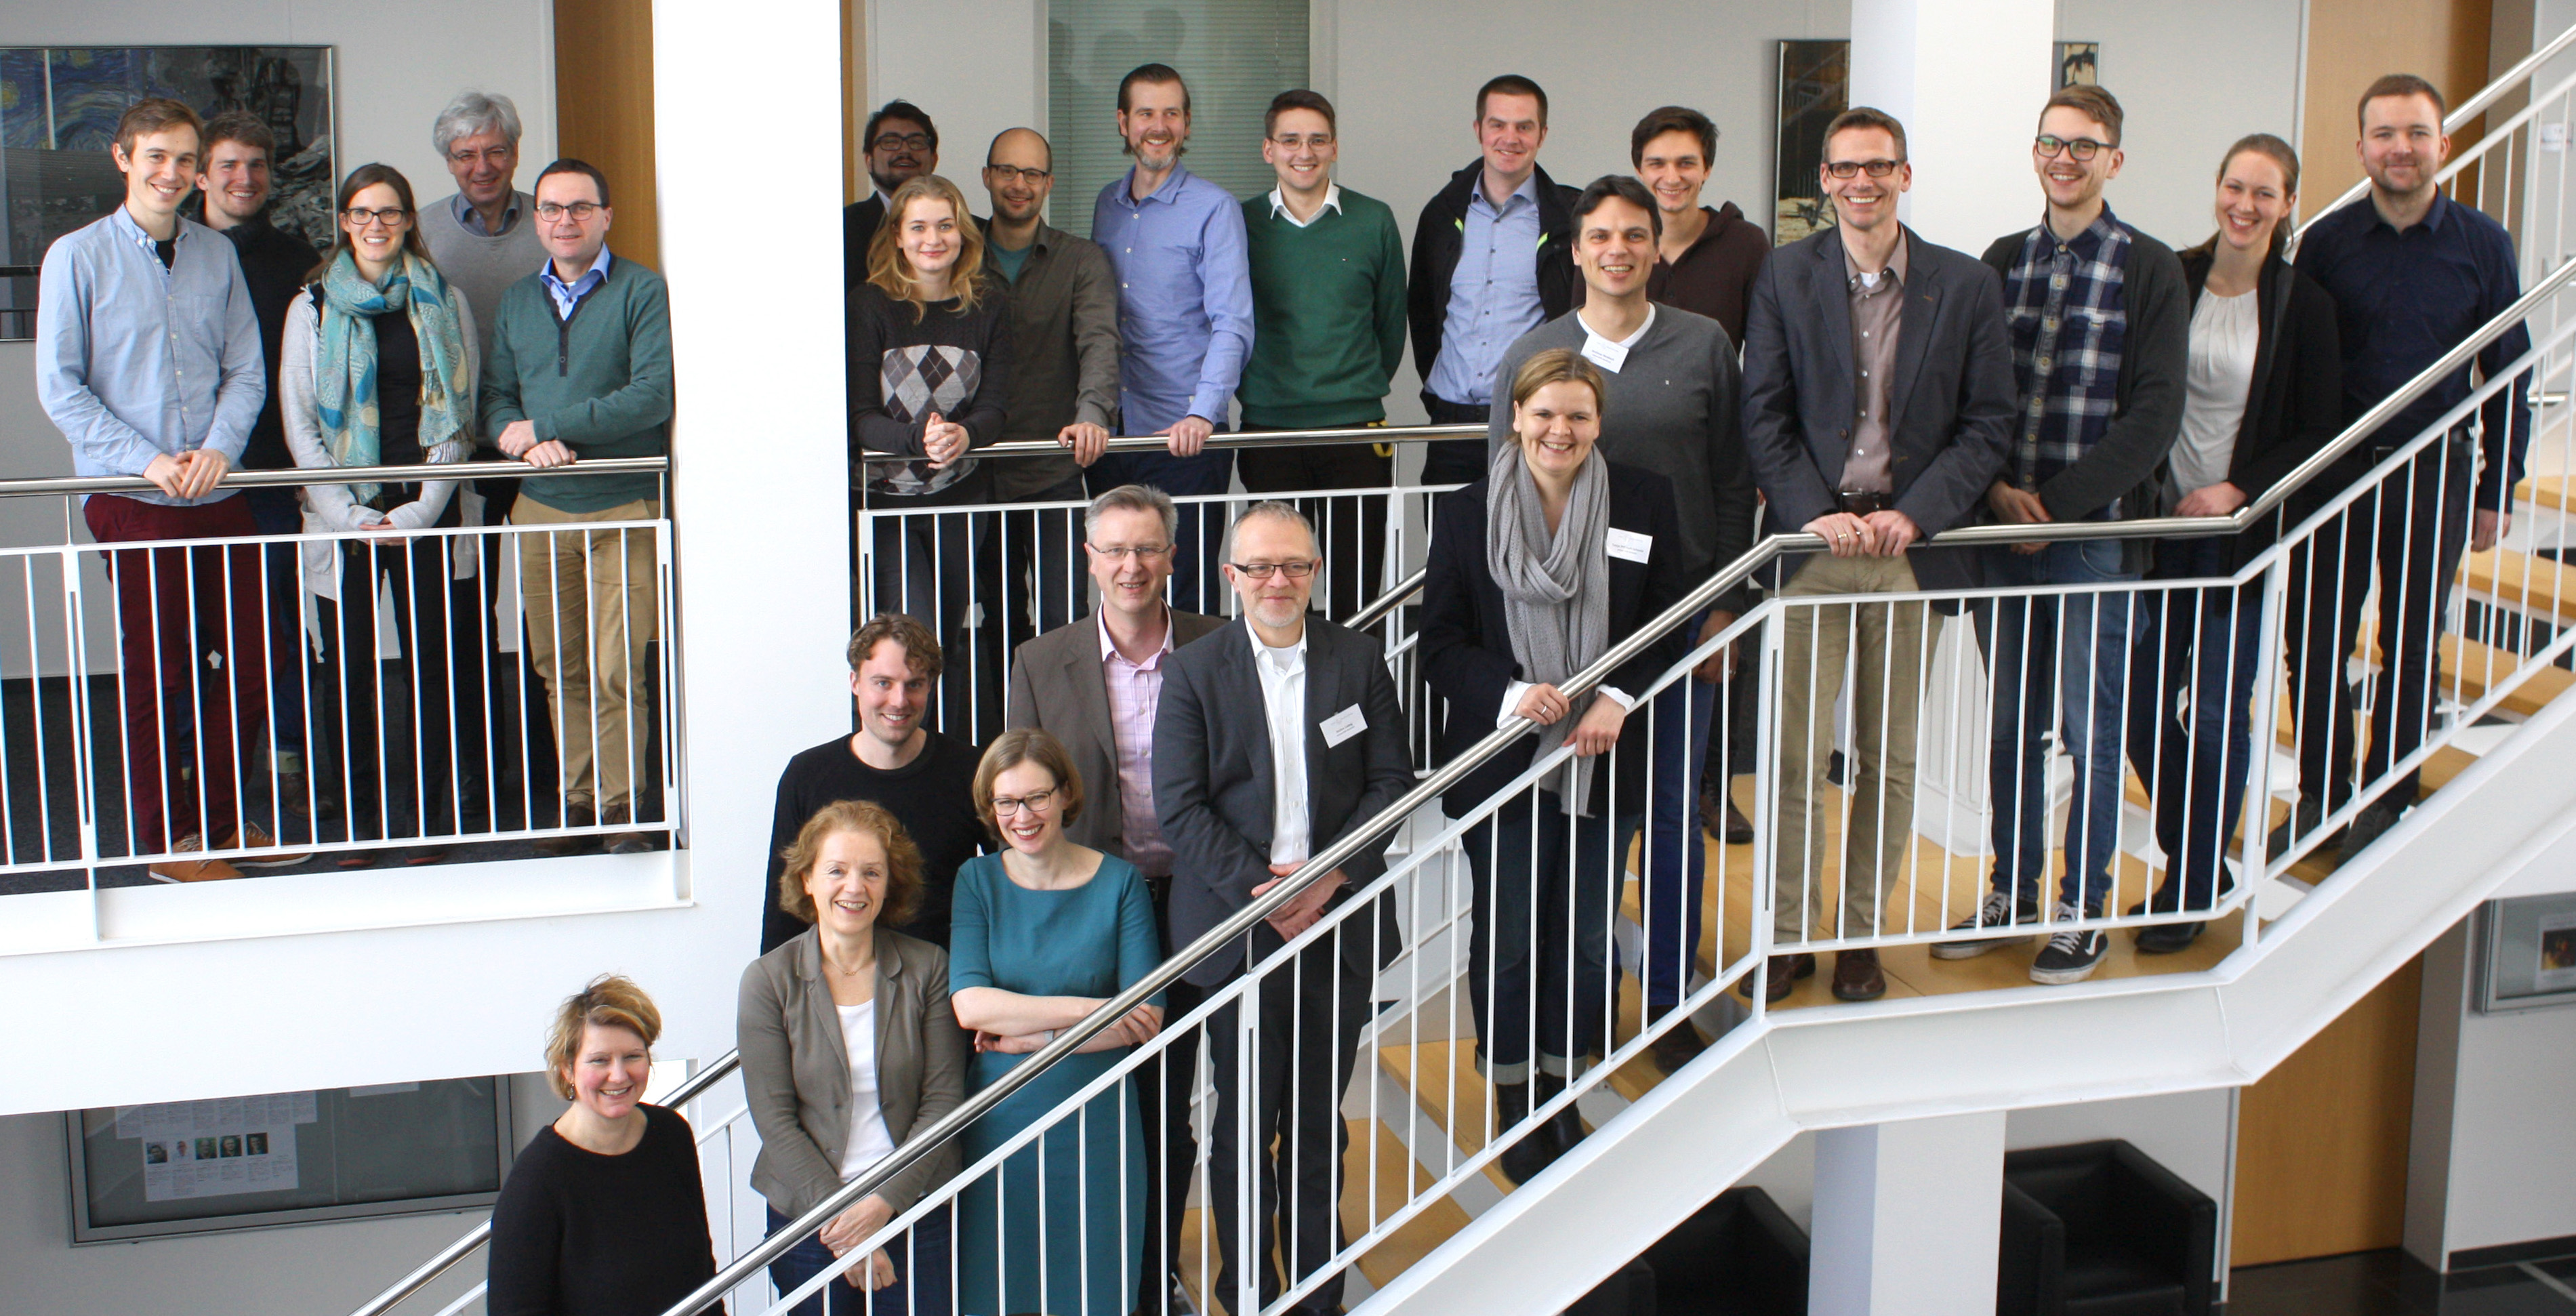
\includegraphics[width=0.85\linewidth]{figures/figure_for.jpg}}
   \end{center}
\end{frame}


%%%%%%%%%%%
% SLIDE 4 %
%%%%%%%%%%%
\begin{frame}{\vspace*{10mm}1\hspace*{1em}Prehistory}
   \textbf{A Tale of Two Working Papers}
   \begin{multicols}{2}
      \begin{center}
         \frame{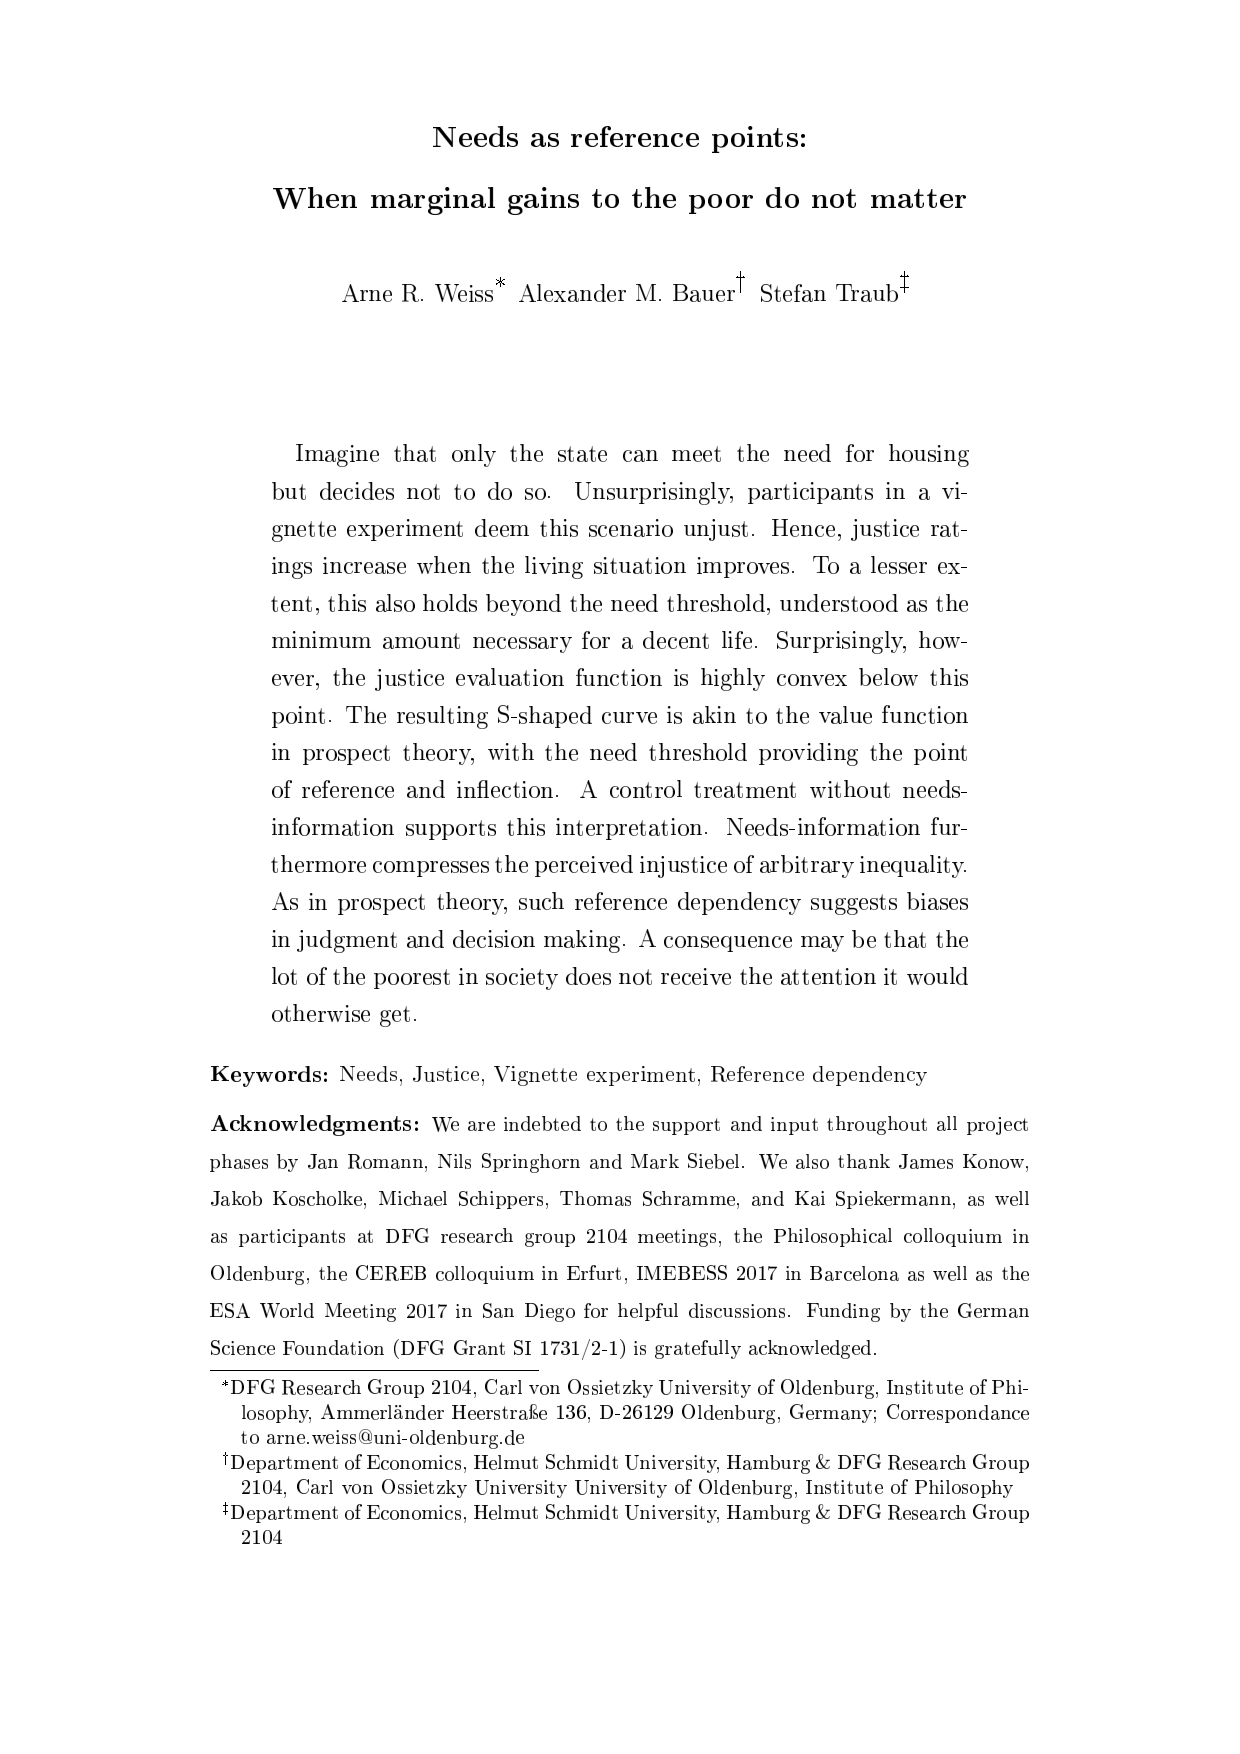
\includegraphics[width=0.5\linewidth]{figures/figure_weiss_2017.pdf}}\\
         \textcolor{gray}{Weiss et al. 2017}\\
         \frame{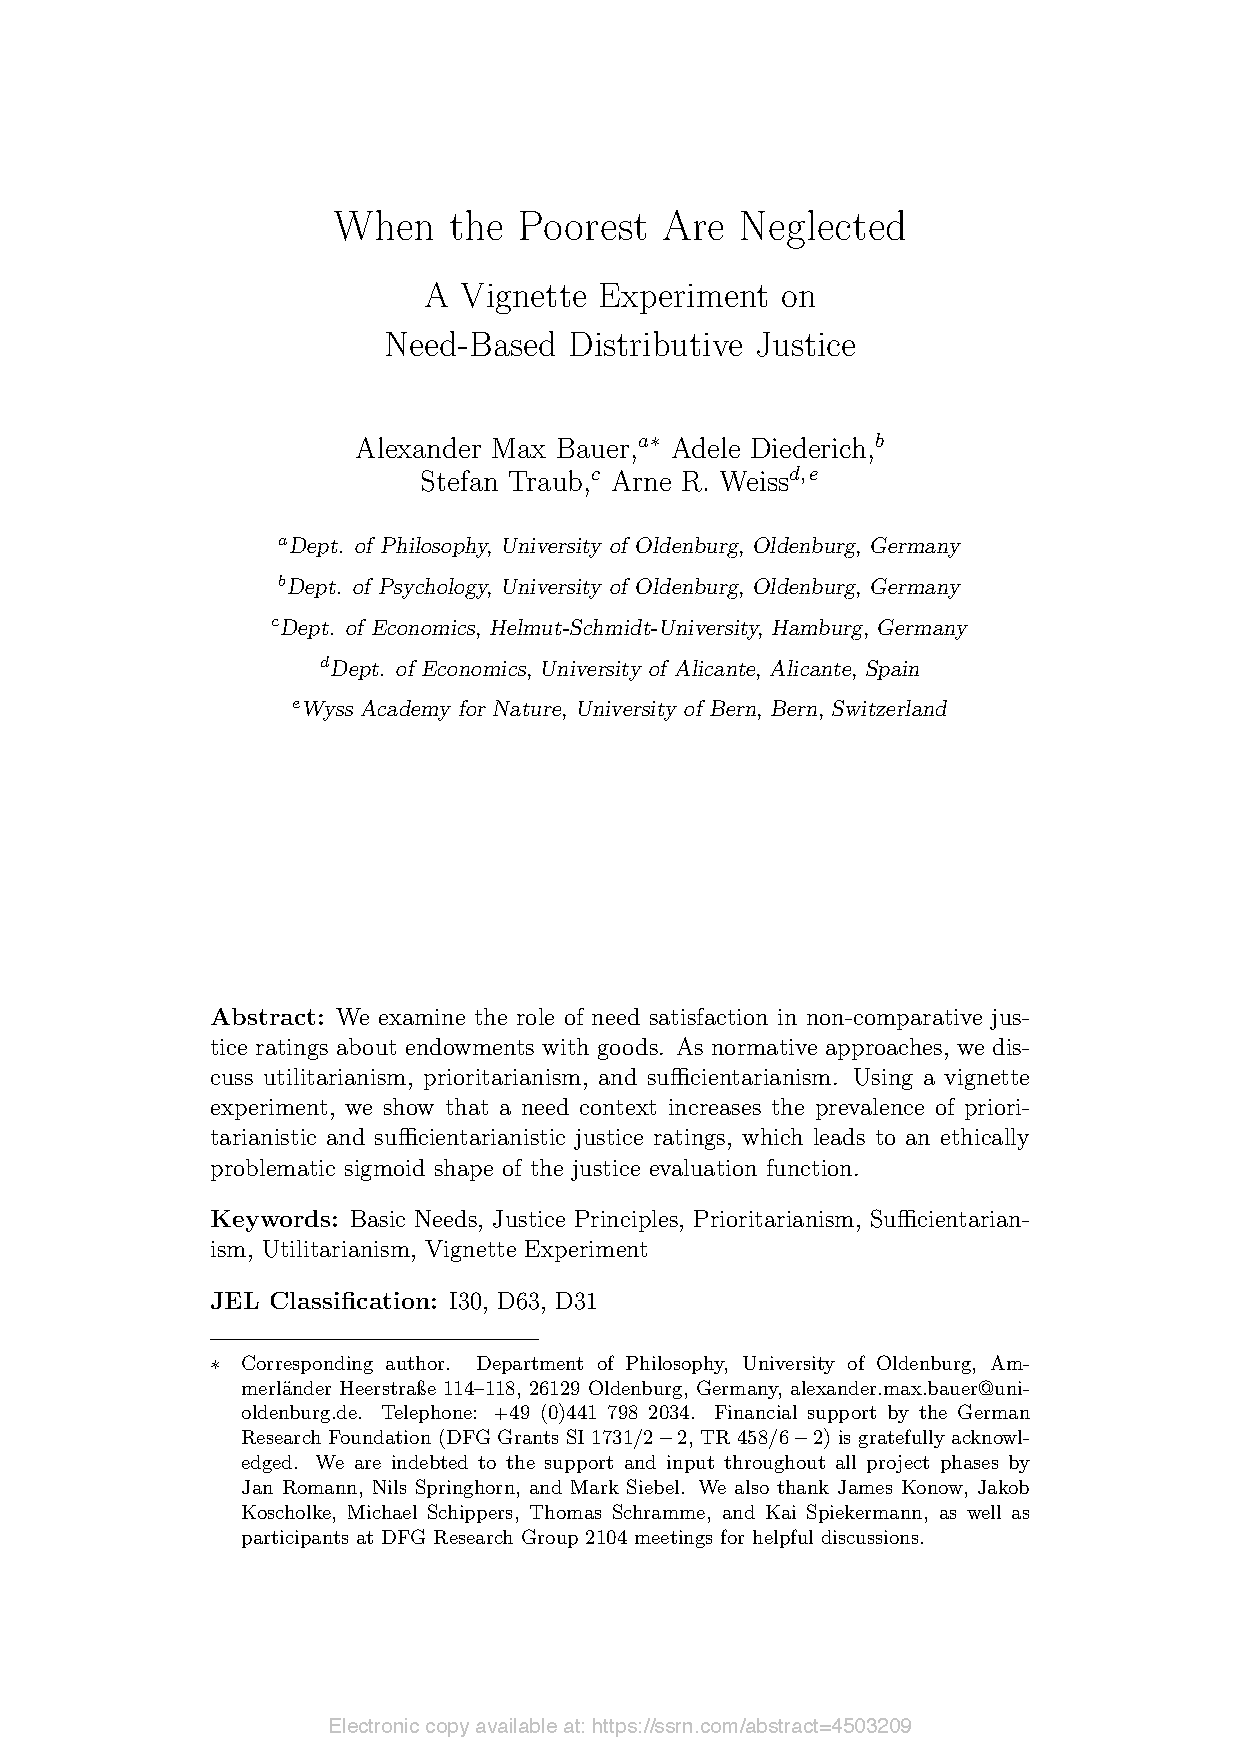
\includegraphics[width=0.5\linewidth]{figures/figure_bauer_2023.pdf}}\\
         \textcolor{gray}{Bauer et al. 2023}\\
      \end{center}
   \end{multicols}
\end{frame}


%%%%%%%%%%%
% SLIDE 5 %
%%%%%%%%%%%
\begin{frame}{\vspace*{10mm}1\hspace*{1em}Prehistory}
   \textbf{Study}
   
   \medskip
   \begin{itemize}
      \item vignette study
      \item two treatments (between-subjects)
      \item two tasks (within-subject)
      \item $n=116$
      \item WiSo experimental laboratory at the University of Hamburg, 2016
      \item role of need satisfaction in non-comparative justice ratings about endowments
      \item justice evaluation function (JEF) as a quantitative measurement of justice evaluations
   \end{itemize}
\end{frame}


%%%%%%%%%%%
% SLIDE 6 %
%%%%%%%%%%%
\begin{frame}{\vspace*{10mm}1\hspace*{1em}Prehistory}
   \textbf{Vignette (1/2)}
   
   \medskip
   Please imagine the following:
   
   \medskip
   In the region of Bergtal, a new village is going to be established.
   It is the task of the Public Housing Association of Bergtal to build housing.
   All households in this region want to live in the largest living space possible.
   \textcolor{blue1}{The residents of the region have collectively decided on a minimum amount of living space, under which living a decent life in this community is not possible.}
   Between the households in the region, there are no noteworthy differences \textcolor{blue1}{and the minimum amounts are the same for each household:
   Each household should have 1000 regional---i.\,e., common to the region---area units of living space in order to be able to live a decent life.
   To have a living space with the equivalent area means for a household to live in close quarters, but it will be just enough to lead a decent life}.
\end{frame}


%%%%%%%%%%%
% SLIDE 7 %
%%%%%%%%%%%
\begin{frame}{\vspace*{10mm}1\hspace*{1em}Prehistory}
   \textbf{Vignette (2/2)}
   
   \medskip
   There are enough means to be able to build up to 2000 regional area units of living space for each household.
   The Regional Parliament decides how much living space will actually be built for the residents of the new village.
   The decision has otherwise no noteworthy consequences.
   For the construction of living space, no additional area would be consumed.
   The new village will be built in the area of an old village that was abandoned after a fire destroyed the houses.
   
   \medskip
   In its decision, the Regional Parliament wants to take into account how impartial people---like you---judge the justice of different scenarios.
   Your task is, therefore, to indicate for each scenario how just you hold the distribution of living space to be.
\end{frame}


%%%%%%%%%%%
% SLIDE 8 %
%%%%%%%%%%%
\begin{frame}{\vspace*{10mm}1\hspace*{1em}Prehistory}
   \textbf{Global Rating Task (1/2)}
   
   \medskip
   The following scenarios differ in how much living space shall be built for each household according to the decision of the Regional Parliament.
   
   \medskip
   Please indicate for each following distribution how just you regard it to be.
   100 percent means that you judge the distribution to be completely just.
   Percentages close to 100 percent mean that you judge the distribution to be almost completely just.
   Percentages far from 100 percent mean that you judge the distribution to be significantly less just.
   
   \medskip
   Please familiarize yourself now with each of the given distributions before answering the questions.
\end{frame}


%%%%%%%%%%%
% SLIDE 9 %
%%%%%%%%%%%
\begin{frame}{\vspace*{10mm}1\hspace*{1em}Prehistory}
   \textbf{Global Rating Task (2/2)}
   \begin{center}
      \frame{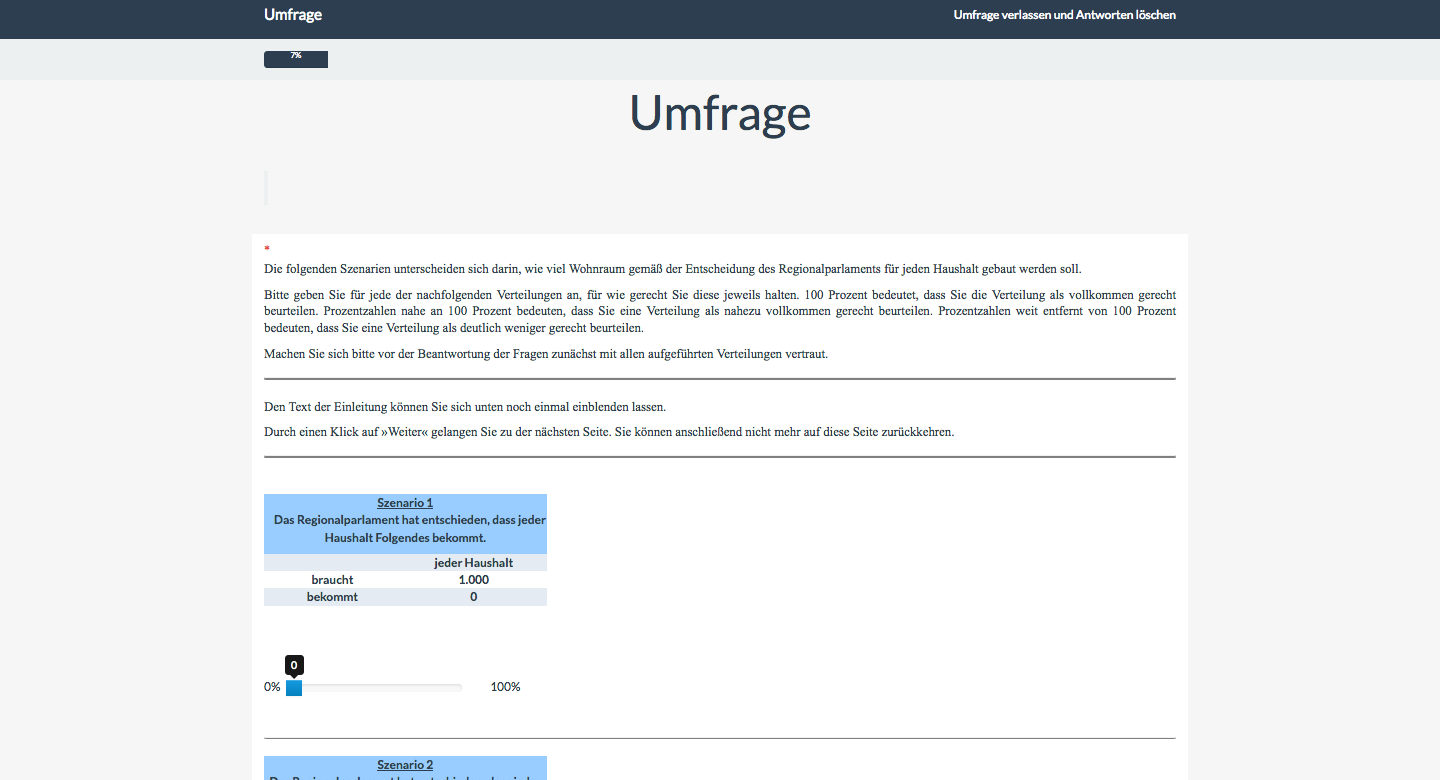
\includegraphics[width=0.75\linewidth]{figures/figure_global_task.png}}
   \end{center}
\end{frame}


%%%%%%%%%%%%
% SLIDE 10 %
%%%%%%%%%%%%
\begin{frame}{\vspace*{10mm}1\hspace*{1em}Prehistory}
   \textbf{Relative Rating Task (1/2)}
   
   \medskip
   On the coming pages, we will present to you each time two differing scenarios.
   We will ask you furthermore to indicate on a scale from 1 (equally just or unjust) to 11 (much more just) how just you regard each scenario compared to the other one to be.
\end{frame}


%%%%%%%%%%%%
% SLIDE 11 %
%%%%%%%%%%%%
\begin{frame}{\vspace*{10mm}1\hspace*{1em}Prehistory}
   \textbf{Relative Rating Task (2/2)}
   \begin{multicols}{2}
      \begin{center}
         \frame{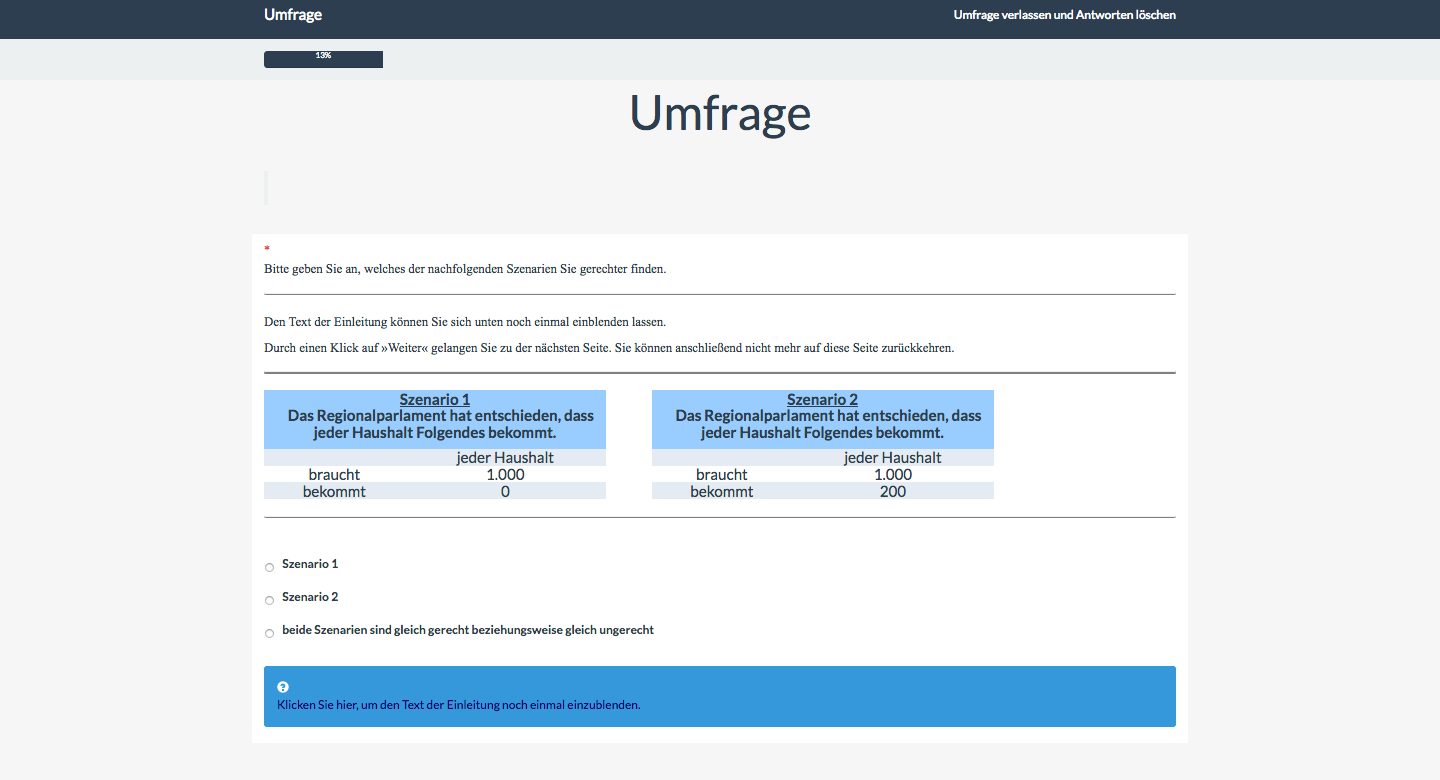
\includegraphics[width=\linewidth]{figures/figure_relative_task_1.png}}
         \frame{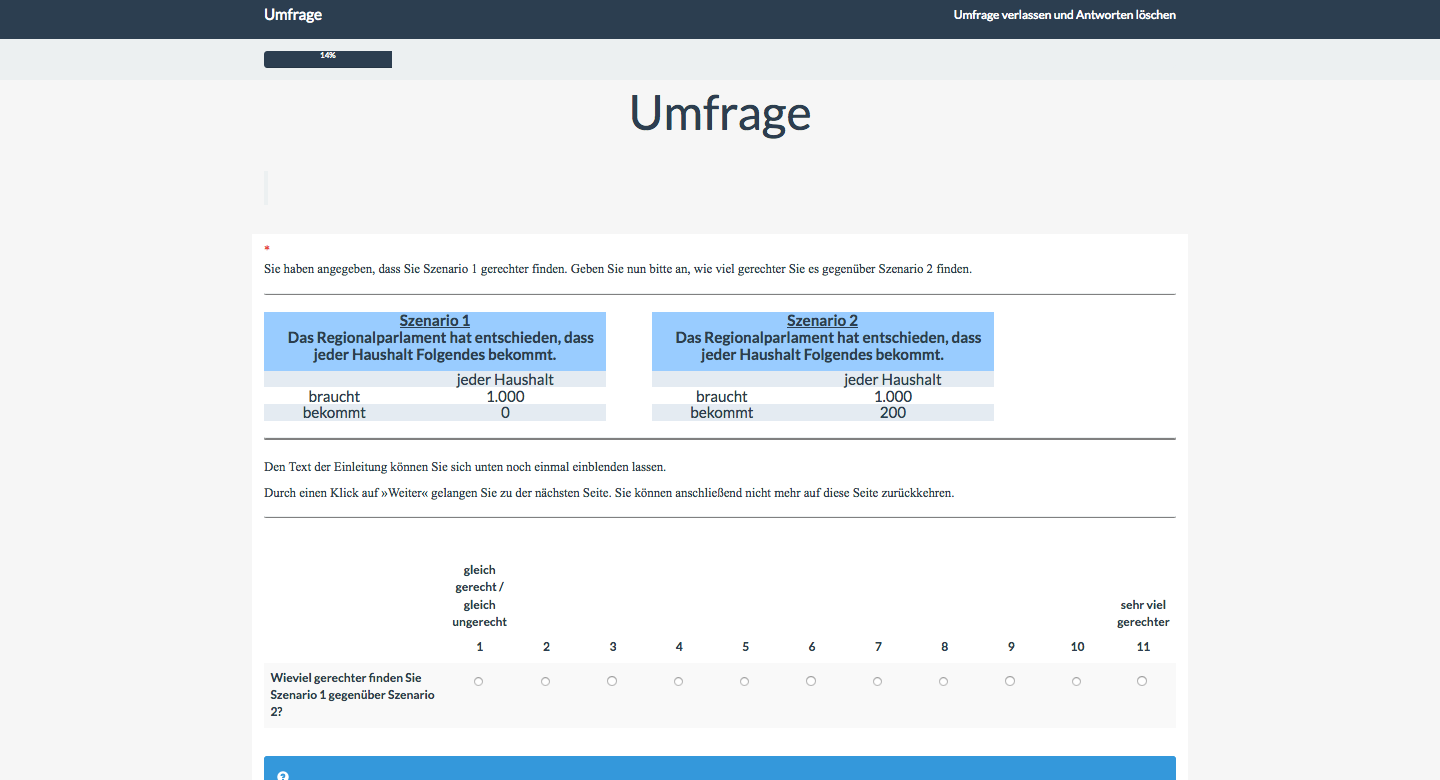
\includegraphics[width=\linewidth]{figures/figure_relative_task_2.png}}
      \end{center}
   \end{multicols}
\end{frame}


%%%%%%%%%%%%
% SLIDE 12 %
%%%%%%%%%%%%
\begin{frame}{\vspace*{10mm}1\hspace*{1em}Prehistory}
   \textbf{Results (1/3)}
   \begin{center}
      \frame{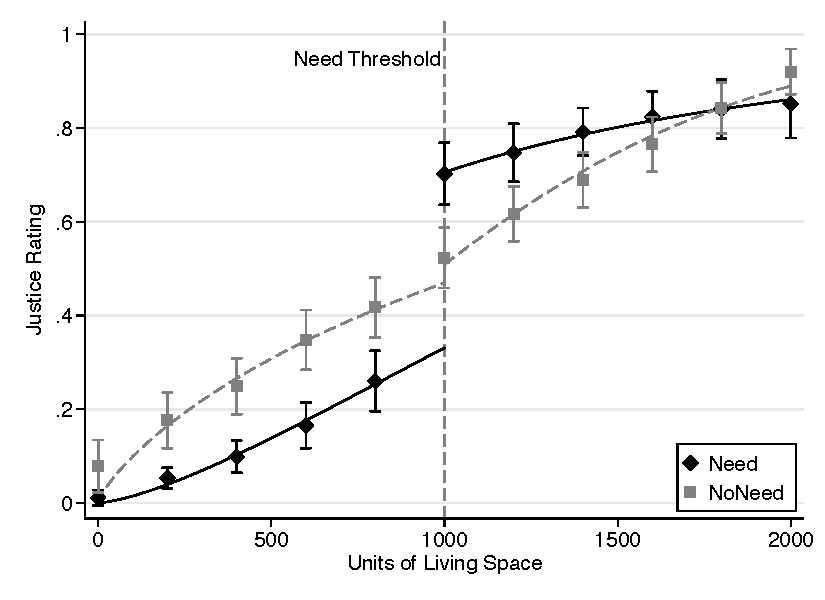
\includegraphics[width=0.5\linewidth]{figures/figure_global_results.pdf}}\\
      \textcolor{gray}{Global Rating Task}
   \end{center}
\end{frame}


%%%%%%%%%%%%
% SLIDE 13 %
%%%%%%%%%%%%
\begin{frame}{\vspace*{10mm}1\hspace*{1em}Prehistory}
   \textbf{Results (2/3)}
   
   \medskip
   \begin{center}
      \begin{tabular}{lrrrr}
         \arrayrulecolor{blue2}\hline
                                        & \multicolumn{2}{c}{Need}   & \multicolumn{2}{c}{NoNeed}   \\
         \hline\hline
         Hump-Shaped                    &  8   &  (15.38\%)          &  2   &   (3.51\%)            \\
         Binary                         &  4   &   (7.69\%)          &  5   &   (8.77\%)            \\
         Flat at/above Need Threshold   &  7   &  (13.46\%)          &  1   &   (1.75\%)            \\
         Zero below Need Threshold      & 15   &  (28.85\%)          &  5   &   (8.77\%)            \\
         Increasing                     & 17   &  (32.69\%)          & 36   &  (63.16\%)            \\
         Other                          &  1   &   (1.92\%)          &  8   &  (14.04\%)            \\
         \hline
                                        & 52   & (100.00\%)          & 57   & (100.00\%)            \\
         \hline
      \end{tabular}
      
      \medskip
      \textcolor{gray}{Global Rating Task}
   \end{center}
\end{frame}


%%%%%%%%%%%%
% SLIDE 14 %
%%%%%%%%%%%%
\begin{frame}{\vspace*{10mm}1\hspace*{1em}Prehistory}
   \textbf{Results (3/3)}
   \begin{center}
      \frame{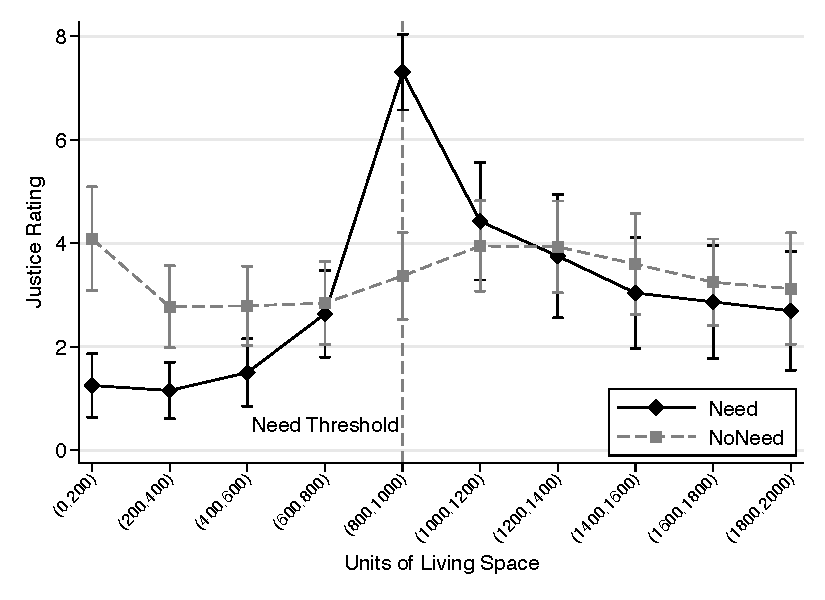
\includegraphics[width=0.5\linewidth]{figures/figure_relative_results.pdf}}\\
      \textcolor{gray}{Relative Rating Task}\\
   \end{center}
\end{frame}


%%%%%%%%%%%%
% SLIDE 15 %
%%%%%%%%%%%%
\begin{frame}{\vspace*{10mm}1\hspace*{1em}Prehistory}
   \textbf{Some Shortcomings}
   
   \medskip
   \begin{itemize}
      \item small and homogeneous sample
      \item no non-normative reference point as control treatment
      \item no separate presentation of scenarios
   \end{itemize}
\end{frame}


%%%%%%%%%%%%%%%%%%%%%%%%%%
% SLIDE 16 – PILOT STUDY %
%%%%%%%%%%%%%%%%%%%%%%%%%%
\begin{frame}
   \begin{overlayarea}{\textwidth}{0.81\paperheight}{
      \vspace*{11mm}
      \usebeamerfont{title}\textcolor{uolblue}
      {2\hspace*{1em}A New Pilot Study}
   }
   \end{overlayarea}
\end{frame}


%%%%%%%%%%%%
% SLIDE 17 %
%%%%%%%%%%%%
\begin{frame}{\vspace*{10mm}2\hspace*{1em}A New Pilot Study}
   \textbf{Vignette (1/2)}
   
   \medskip
   Please imagine the following:
   
   \medskip
   The Müller family has a certain need for living space.
   That means they require an apartment with a specific number of square meters in order to live in decency.
   If they receive exactly this number of square meters, their need for living space is exactly met.
   If they receive less, their need is underfulfilled.
   If they receive more, their need is overfulfilled.
   The Müller family requires 100 square meters.
   On the next page, we will show you various scenarios in which the actual size of the apartment they receive differs.
\end{frame}


%%%%%%%%%%%%
% SLIDE 18 %
%%%%%%%%%%%%
\begin{frame}{\vspace*{10mm}2\hspace*{1em}A New Pilot Study}
   \textbf{Vignette (2/2)}
   
   \medskip
   Please evaluate how well the number of square meters fulfil the Müller family's need in each case \textcolor{blue1}{[how just the number of square meters is in regard to the Müller family's need in each case]}.
   You can do this by providing a number.
   0 indicate that their need is exactly fulfilled \textcolor{blue1}{[that they receive a just amount]}.
   Negative values indicate that their need is underfulfilled \textcolor{blue1}{[that they receive less than would be just]}.
   Positive values indicate that their need is overfulfilled \textcolor{blue1}{[that they receive more than would be just.]}.
   The more strongly the need is under- or overfulfilled \textcolor{blue1}{[the allocation deviates from what is fair]}, the higher the value should be.
   Please base your judgments on your own personal assessment.
   There are no right or wrong answers.
\end{frame}


%%%%%%%%%%%%
% SLIDE 19 %
%%%%%%%%%%%%
\begin{frame}{\vspace*{10mm}2\hspace*{1em}A New Pilot Study}
   \textbf{Task}
   \begin{center}
      \frame{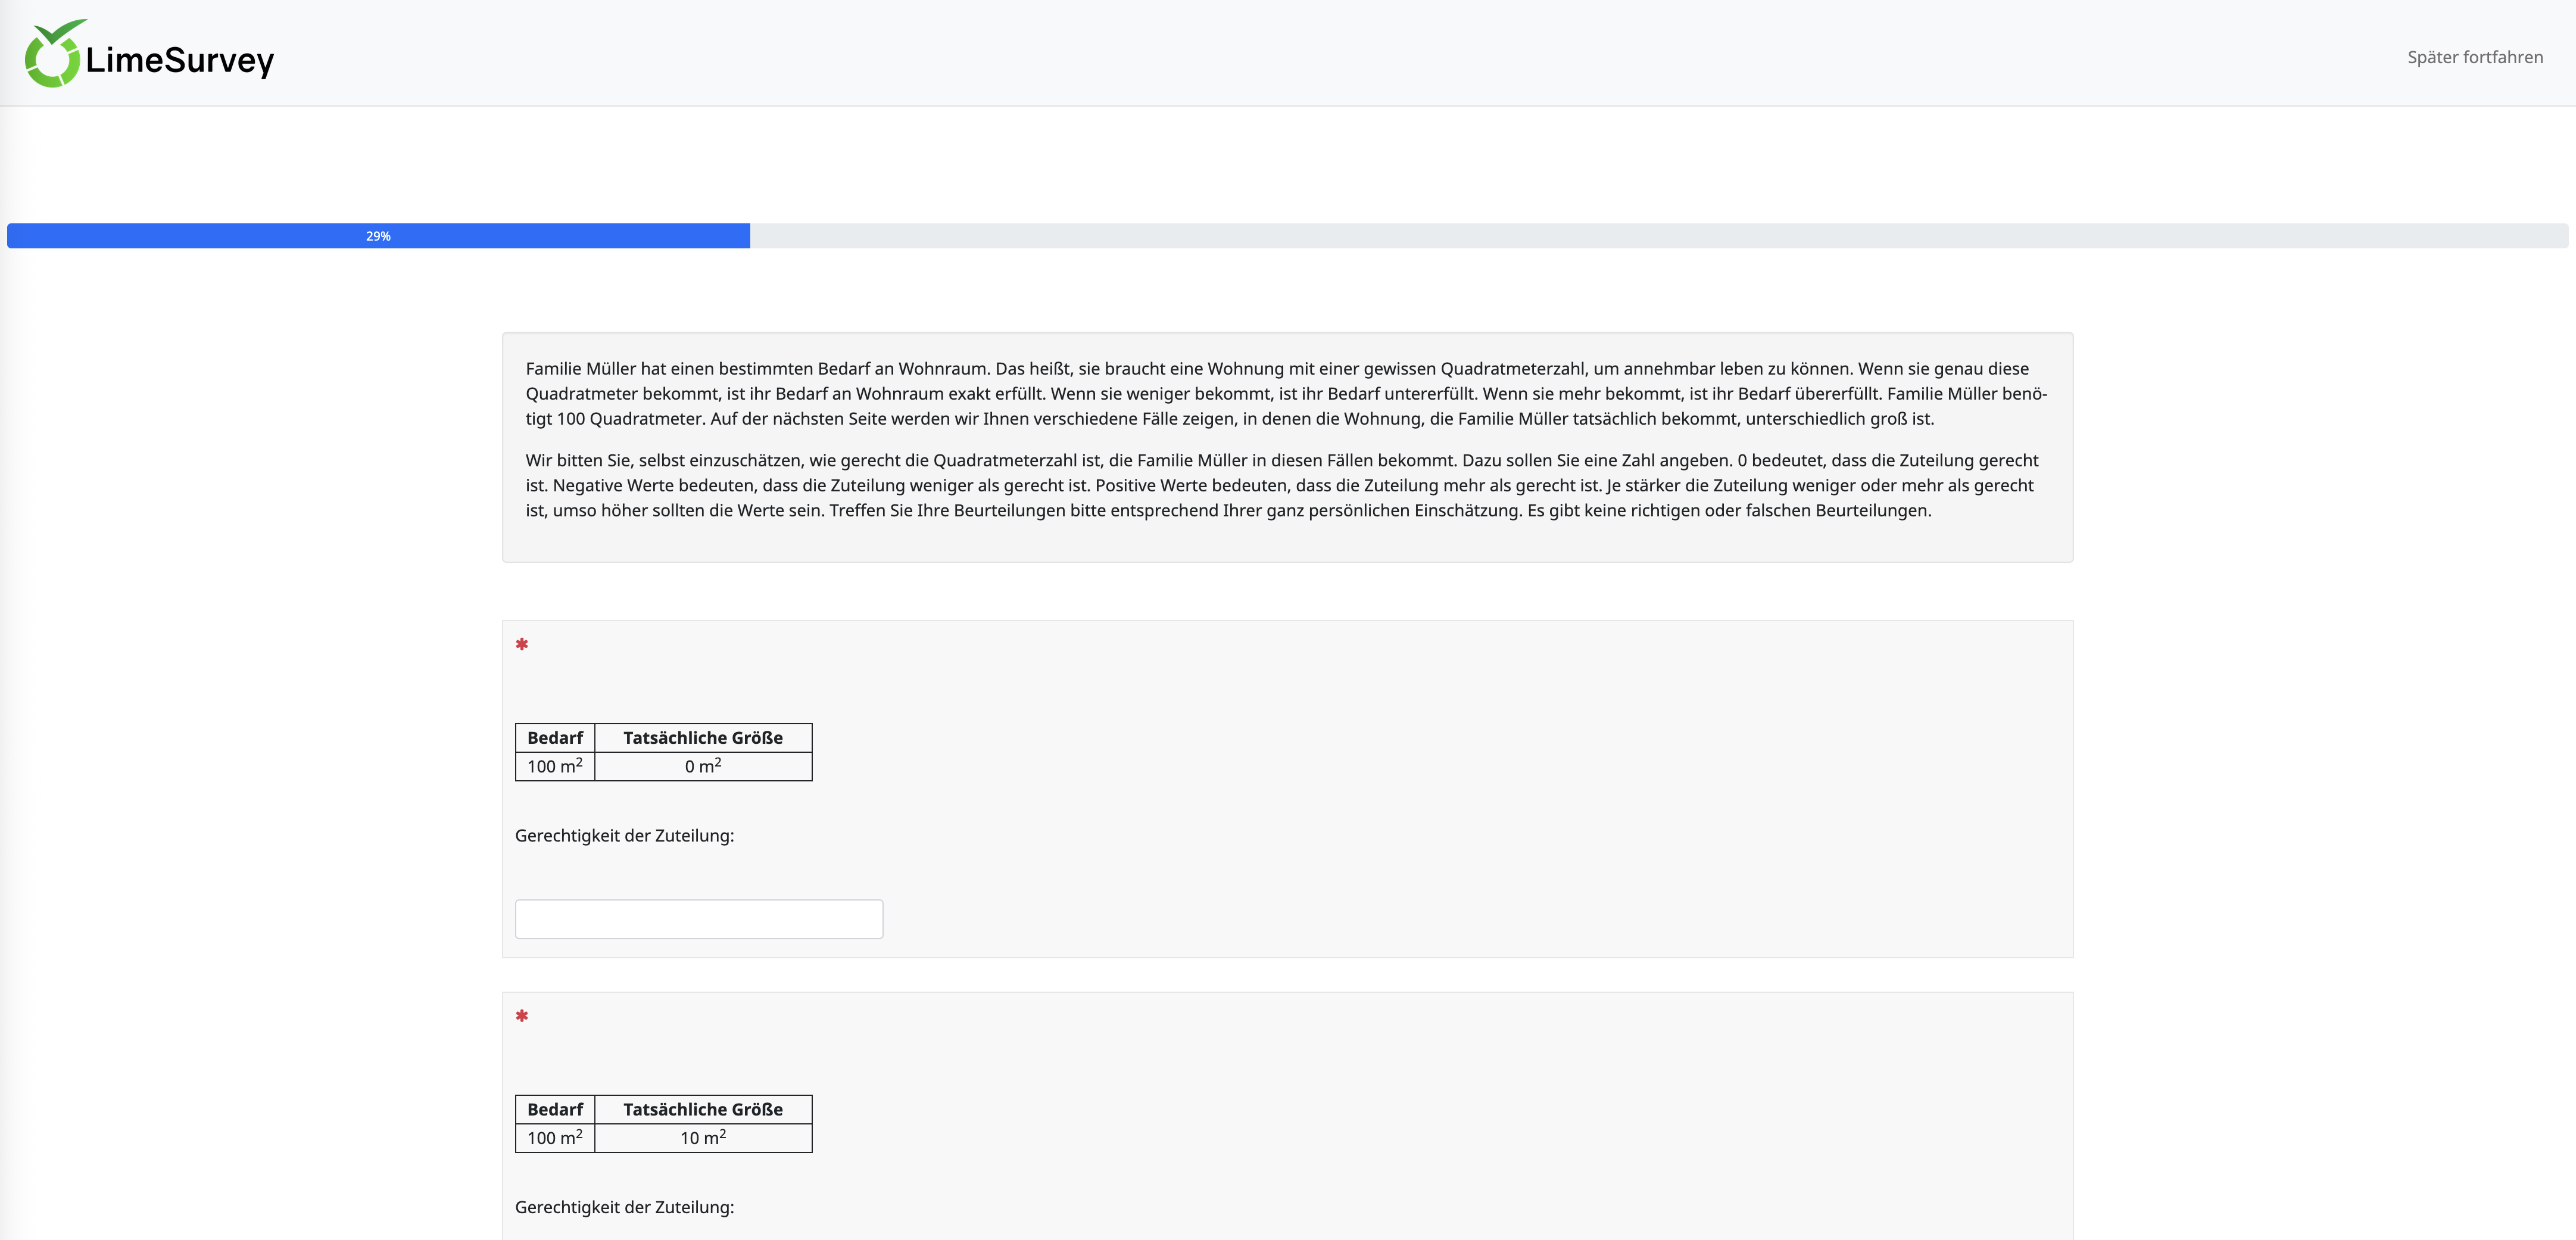
\includegraphics[width=0.75\linewidth]{figures/figure_pilot_task.png}}\\
      \textcolor{gray}{Relative Rating Task}
   \end{center}
\end{frame}


%%%%%%%%%%%%
% SLIDE 20 %
%%%%%%%%%%%%
\begin{frame}{\vspace*{10mm}2\hspace*{1em}A New Pilot Study}
   \textbf{Results}
   \begin{multicols}{2}
      \begin{center}
         \frame{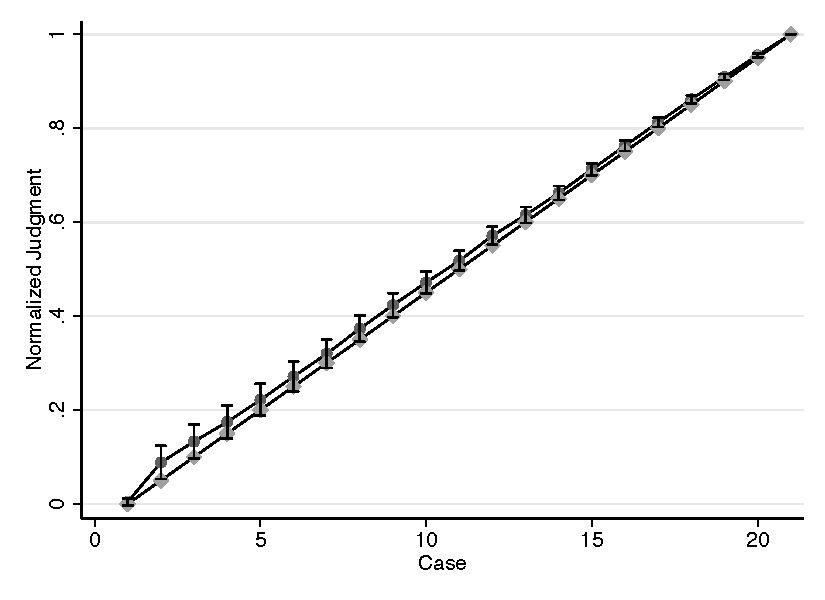
\includegraphics[width=\linewidth]{figures/figure_pilot_results_1_1.pdf}}\\
         \textcolor{gray}{Non-Normative Formulation\\($n=74$)}\\
         \frame{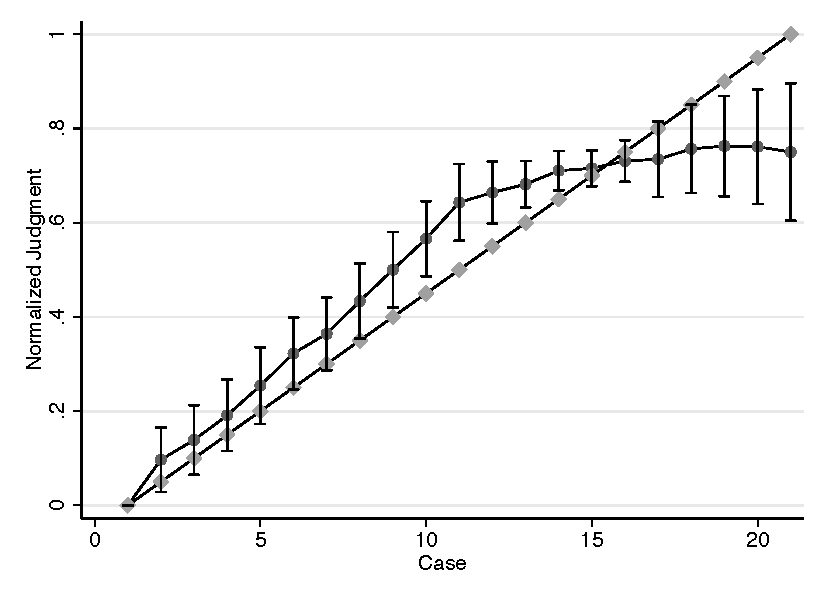
\includegraphics[width=\linewidth]{figures/figure_pilot_results_3_1.pdf}}\\
         \textcolor{gray}{Normative Formulation\\($n=24$)}\\
      \end{center}
   \end{multicols}
\end{frame}


%%%%%%%%%%%%
% SLIDE 21 %
%%%%%%%%%%%%%
\begin{frame}
   \begin{overlayarea}{\textwidth}{0.81\paperheight}{
      \vspace*{11mm}
      \usebeamerfont{title}\textcolor{uolblue}
      {3\hspace*{1em}Some Ideas}
   }
   \end{overlayarea}
\end{frame}


%%%%%%%%%%%%
% SLIDE 22 %
%%%%%%%%%%%%
\begin{frame}{\vspace*{10mm}3\hspace*{1em}Some Ideas}
   \textbf{Takeaway Points}
   
   \medskip
   \begin{itemize}
      \item presence of a need-based reference point alters the sense of what is fair
      \item[] \textcolor{gray}{(Weiss et al. 2017, Bauer et al. 2023)}
      \item not merely the existence of a reference point matters---but its normative framing
      \item[] \textcolor{gray}{(pilot study)}
   \end{itemize}
\end{frame}


%%%%%%%%%%%%
% SLIDE 23 %
%%%%%%%%%%%%
\begin{frame}{\vspace*{10mm}3\hspace*{1em}Some Ideas}
   \textbf{Potential Directions for Future Research}
   
   \medskip
   \begin{itemize}
      \item How do reference points affect evaluations of distributive justice? \textcolor{gray}{(descriptive)}
      \begin{itemize}
         \item various (isolated) (non)normative reference points
         \item multiple (competing) (non)normative reference points
      \end{itemize}
      \item What is the cognitive nature of such evaluations? \textcolor{gray}{(explanatory)}
      \begin{itemize}
         \item (in)consistencies of evaluations
         \item intuitive evaluations versus evaluations with reflective interventions
         \item evaluations under time pressure, cognitive load, or distraction (dual process)
         \item cross-population or cross-cultural influences
      \end{itemize}
   \end{itemize}
\end{frame}


%%%%%%%%%%%%
% FOLIE 24 %
%%%%%%%%%%%%
\begin{frame}{\vspace*{10mm}References}
   \vspace*{-10mm}
   {\footnotesize
   \begin{itemize}[label=,leftmargin=2em,itemindent=-2em]
      \item Bauer, Alexander Max, Adele Diederich, Stefan Traub, and Arne Robert Weiss (2023): \enquote{Thinking About Need. A Vignette Experiment on Need-Based Distributive Justice,} \textit{SSRN Working Paper} 4503209. \url{https://papers.ssrn.com/sol3/papers.cfm?abstract_id=4503209}
      \item Weiss, Arne Robert, Alexander Max Bauer, and Stefan Traub (2017): \enquote{Needs as Reference Points. When Marginal Gains to the Poor do not Matter,} \textit{FOR 2104 Working Paper} 2017-13. \url{https://www.hsu-hh.de/bedarfsgerechtigkeit/wp-content/uploads/sites/857/2021/03/2017-13.pdf}
   \end{itemize}
   }
\end{frame}


\end{document}
